\section{Experimental Results}

We now present the experimental results obtained on the dataset. 
The initial ones obtained with a random train test split, more specifically, 
70\% percent of the dataset is considered for the training, while the remaining part
for test. 
Out of that 70\%, a random 20\% is used for validation purposes.

\subsection{Training without augmentation}

After splitting the dataset randomly, SVM, K-NN and a Decision tree are trained and evaluated.
Those models do not perform really well compared to the neural networks in use.

The MLP and the CNN are trained with fit parameters on default, the number of epochs is quite high as
the learning rate for the optimizer is low to prevent a local minimum, they are 
1000 and 1500 respectively. The best model in terms of validation accuracy is saved 
and later loaded to obtain the accuracy results.

One factor in the training of the neural networks are the class weights. As can be seen 
in figure \ref{fig:classes}, there is a slight unbalance in the classes of the 
dataset. This would lead to poor performance on the under represented ones, thus 
class weights are computed and used during training.

The training results of the models can be seen in Table \ref{tab:res1}. 
MLP outperform other methods, while neural networks works better than simpler models.

\begin{table}
    \begin{center}
        \begin{tabular}{ |l|r| } 
        \hline
        Model & Accuracy \\
        \hline
        SVM   & 0.574 \\
        K-NN   & 0.400 \\
        Dtree & 0.381 \\
        MLP   & 0.645 \\
        CNN   & 0.633 \\
        \hline
        \end{tabular}
    \end{center}
    \caption{Training results without data augmentation.} \label{tab:res1}
\end{table}

\begin{figure}
    \begin{center}
      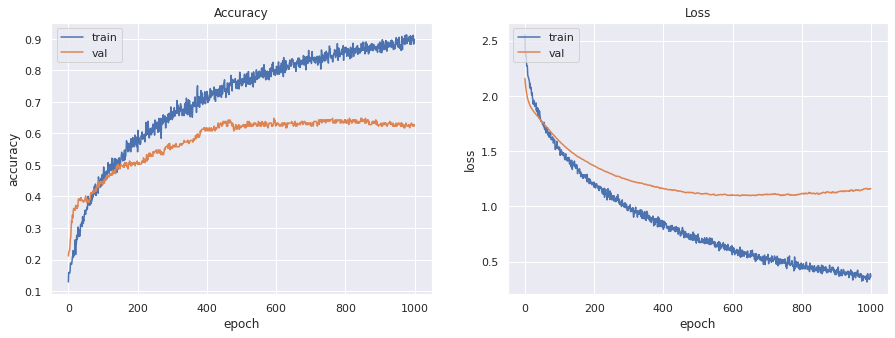
\includegraphics[width=\textwidth]{images/mlp1.png}
      \caption{Multilayer perceptron training progress on non-augmented data. Despite the 
      high number of epochs, dropout and a slow 
      learning rate prevents overfitting, as it only begin around epoch 600, 
      when the validation error start increasing.} \label{fig:mlp1}
    \end{center}
\end{figure}

\subsection{Training with data augmentation}

After testing the models without augmentation, speed, noise and pitch augmenters 
are used on the training set to enlarge it. 
As said before, the augmented data is used only on the training and validation set, 
while the randomly drawn test set remains in the original state.
The setup is exactly the same as before, so results can be compared. 
They can be seen in Table \ref{tab:res2}.

\begin{table}[H]
    \begin{center}
        \begin{tabular}{ |l|r|r| } 
        \hline
        Model & Accuracy w/o aug. & Accuracy w/ aug. \\
        \hline
        SVM   & 0.574  &  0.631 \\
        K-NN   & 0.400  &  0.414 \\
        Dtree & 0.381  &  0.428 \\
        MLP   & 0.645  &  0.659 \\
        CNN   & 0.633  &  0.668 \\
        \hline
        \end{tabular}
    \end{center}
    \caption{Training results with data augmentation.} \label{tab:res2}
\end{table}

\noindent Overall, every model performs better with data augmentation, the CNN is the best 
one, closely followed by MLP. An interesting note is that SVM with data augmentation 
has similar performances to CNN without data augmentation.

\subsection{Cross validation results}

The preliminary test on training with and without augmentation 
gives an idea about model performances, but to better evaluate them cross validation 
is required. 

The idea is to split the dataset in $K$ splits, train a model on $K-1$ splits
and evaluate on the latter. The process is repeated $K$ times and mean and standard deviation for
accuracy are computed. 
In this case, stratified cross validation with five folds is used. The stratified
version keeps in mind classes cardinalities when splitting the dataset, 
ensuring a similar distribution across all splits.
This method gives a better statistical estimation of the accuracy and loss, as 
splitting only once and obtaining a good results can be mostly luck-related.


To evaluate the impact of data augmentation, only the training splits are augmented, 
leaving the test split untouched, results can be seen in table \ref{tab:res3}.
The quantity in the parenthesis is the standard deviation.

\begin{table}[H]
    \begin{center}
        \begin{tabular}{ |l|r|r| } 
        \hline
        Model & Mean acc. w/o aug. (std) & Mean acc. w/ aug. (std)\\
        \hline
        SVM   &  0.588 (0.035)  &  0.643 (0.015) \\
        K-NN  &  0.441 (0.023)  &  0.422 (0.016) \\
        Dtree &  0.403 (0.036)  &  0.421 (0.041) \\
        MLP   &  0.611 (0.031)  &  0.692 (0.012) \\
        CNN   &  0.490 (0.058)  &  0.698 (0.030) \\
        \hline
        \end{tabular}
    \end{center}
    \caption{Cross validation results.} \label{tab:res3}
\end{table}

\noindent Again, data augmentation improves accuracy, but we can also see that the standard deviation is reduced
almost in all cases.
Also, the mean accuracy for CNN without data augmentation is drastically low 
with respect to the preliminary results obtained on the dataset, highlighting the importance
of performing cross validation.

\section{Concluding remarks}

This study explored audio speech emotion classification, comparing 
models trained on handcrafted features, and CNNs on MFCC.
A focus is putted on data augmentation and the results 
show how this procedure increases performance by a lot. 
Finally, cross validation is used to rank models between themselves.

Some possible future works involves exploring with additional 
augmentation, finding how much more data we can build from the dataset. 
Other models could be explored, like auto-encoders or LSTMs, as 
they perform really well on audio.